\chapter{Frequency and Scale}

\section{Thinking in Frequency: Fourier Transform}
\subsection{Hybrid images}
How does it work? Take low freq. content from one image and high freq content from another. On long distance humans can see only low frequency content.

\textbf{Fouriers idea}: Any univariate function can be rewritten as a weighted sum of sines and cosines of different frequencies.

\subsection{Waves in 2D} A 2D wave for an image is given as $f(x,y) = r \cos(2\pi (\omega_x x + \omega_y y) + \phi)$, $\omega = [\omega_x \omega_y]$ being the \textbf{wave number}, $f = |\omega|_2$ the frequency, $\omega /f$ the direction of the wave and $\phi$ the phase, $r$ the amplitude. 

Examples are given by

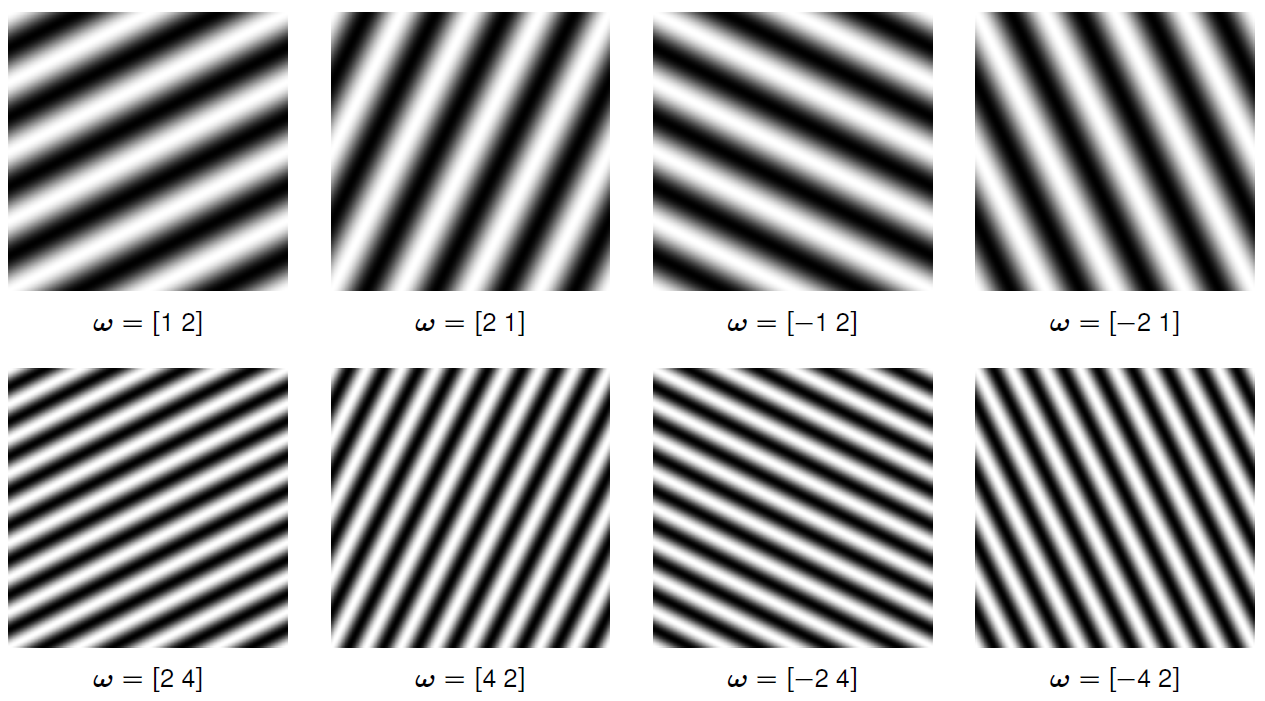
\includegraphics[width=.7\textwidth]{images/chap4/freq_examples}, varying the phase, shifts the signals position.

\textbf{Complex elementary wave}: For $\omega = [\omega_x \omega_y]$, $W_\omega (p) = e^{2\pi i (\omega p)} = \cos(2\pi(\omega p)) + i \sin(2\pi (\omega p))$, with phase zero, amp. one.

\textbf{Central idea of fourier transform:}

\begin{align*}
    f(p) & = \int_{\mathbb{R}^2} \hat{f}(\omega) W_\omega (p) d\omega \\
    & = \int_{\mathbb{R}}\int_{\mathbb{R}} \hat{f} (\omega_x, \omega_y) e^{2\pi i(\omega_x x + \omega_y y)} d\omega_x d\omega_y
\end{align*}, $\hat{f}$ being the fourier transform of $f$.

\textbf{Observations:}

\begin{itemize}
    \item Sum of signals, is sum of fourier transforms
    \item Getting rid of imag. part in a complex wave, is adding it with it's conjugate
    \item Noise amplifies large frequencies
    \item Cutting out a section of the fourier transform is similar to blurring (Low-pass)
    \item Phase is more important for how a picture looks like
\end{itemize}

\textbf{Inner product of complex numbers z,w:} Multiply $z$ b y comp. conjugate of $w$! (Hermitian inner product).

\textbf{Inner product for function $f,g: \mathbb{R}^2 \rightarrow \mathbb{C}$}: $(f,g)_{\mathbb{C}}$ is a function as a vector with infinitely many components. Summing over components becomes an integral and we get 
\begin{align*}
    (f,g)_{\mathbb{C}} & = \int_{\mathbb{R}^2} f(p) \overline{g}(p) dp \\
    & = \int_{\mathbb{R}}\int_{\mathbb{R}} f(x,y) \overline{g}(x,y) dx dy
\end{align*}

The \textbf{fourier coefficients} are then defined as:
\begin{align*}
    \hat{f}(\omega) & = (f,W_\omega)_{\mathbb{C}}\\
    & = \int_{\mathbb{R}^2} f(p) \overline{W}_\omega(p) dp \\
    & = \int_{\mathbb{R}}\int_{\mathbb{R}} f(x,y) e^{-2\pi i(\omega_x x + \omega_y y)} dx dy
\end{align*}

\section{Filtering in frequency space}

\subsection{Shifting theorem and convolution theorem}

Shifting a wave by vector $p_0$ results in a phase shift by $2\pi \omega \cdot p_0$,i.e., $e^{2\pi i \omega p} e^{-2\pi i \omega p_0} = e^{2\pi i \omega (p-p_0)}$. For the \textbf{FT} this means shifting by a vector $p_0$ means shifting all elementary waves by $e^{-2\pi i \omega \cdot p_0}$.

\textbf{Convolution:} Is the same as multipliying the corresponding elementary waves one by one. Hence $\hat{f * g} = \hat{f} \hat{g}$.

The \textbf{FT} of a gaussian is a gaussian-like function. When looking at the image, one can see that it corresponds to a low-pass filter.

\begin{itemize}
    \item Low-pass: gaussian
    \item High-pass: Impulse minus gaussian
    \item Band-pass: Difference of gaussians
\end{itemize}

\subsection{Derivatives and the fourier transform}

Taking derivatives amplifies high frequencies, higher frequency and derivative order, higher amplification.

\begin{align*}
    \partial_x^n\partial_y^m f(p) & = \int_{\mathbb{R}}\int_{\mathbb{R}} \hat{f}(\omega) \partial_x^n\partial_y^m[e^{2\pi i(\omega_x x + \omega_y y)}] dx dy \\
    & = \int_{\mathbb{R}^2} (2\pi i \omega_x)^n (2\pi i \omega_y)^m \hat{f}(\omega) W_\omega (p) dp \\
 \hat{\partial_x^n\partial_y^m} f(\omega) & = (2\pi i \omega_x)^n (2\pi i \omega_y)^m \hat{f}(\omega)
\end{align*}

\textbf{Properties of the FT:}

\begin{itemize}
    \item Linearity: Constant factor and additive
    \item Rotation invariant: Rotation of $f$ means rotation of $\hat{f}$ (same angle)
    \item Shift theorem
    \item Convolution theorem
    \item Derivatives
\end{itemize}

\section{Sampling and image pyramids}

\subsection{Sampling and aliasing}

Remember, naively finding a patch is not scale invariant. If the image has too many pixels compared to a patch we need to downsample the image, since both patch and image resolution have to be the same.

\textbf{Sampling theorem:} $f$ band-limited, i.e., highest frequency $W$ exists with $\hat{f} (\omega) = 0 if |\omega|_2 > W$. The sampling rate has to be twice as high.

For sampling distance $h$ this means $h < h_{max} = 1/2W$.

\textbf{Downsampling:} Depending on the highest frequency in the image, at a certain point we get aliasing. Downsampling means reducing sampling distance $h$, reducing nyquist frequency as well.

\textbf{Solution:} Band-limit signal further before down sampling.

\subsection{Gaussian pyramids}

Gaussian prefiltering: blur $\rightarrow$ downsample $\rightarrow$ blur $\rightarrow \dots$.

\textbf{Gaussian pyramid:} Represent $N\times N$ image as subimages of powers of 2 resulting in a pyramid:

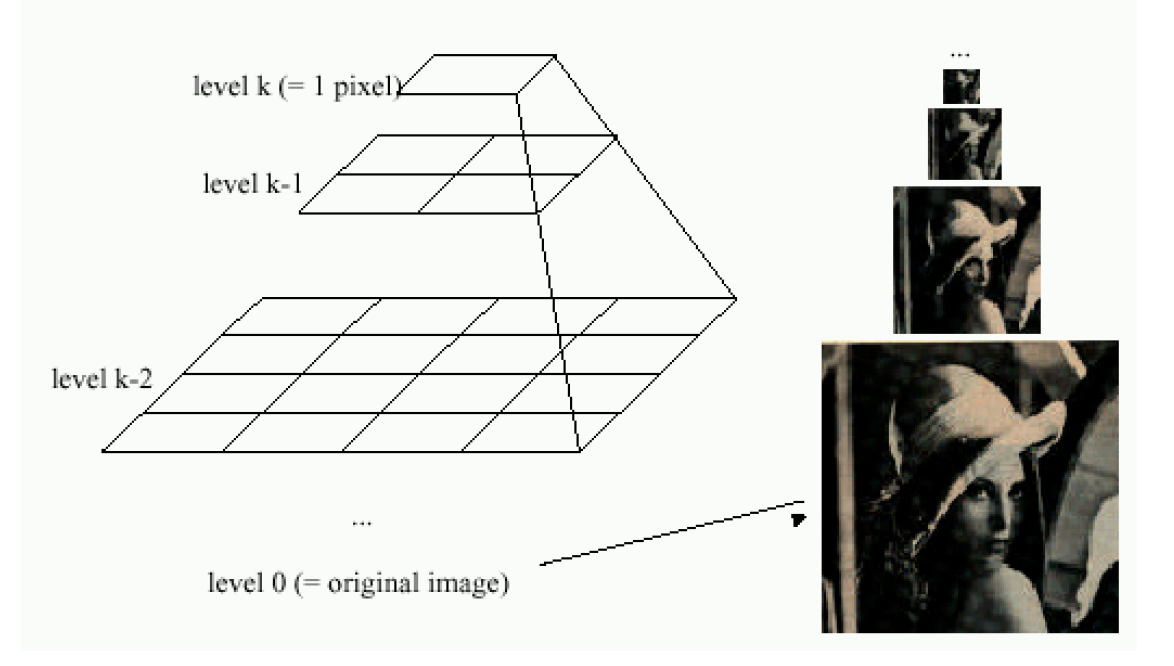
\includegraphics[width=.7\textwidth]{images/chap4/gaus_pyra}

For this we have approx. $4/3$ storage space requirement.

\subsection{Laplacian pyramids}

Different idea: Instead of storing the full image at subsequent levels, we store the high-frequency content, i.e. the difference of gaussians at each level.

\section{Summary}

\textbf{FT:}

\begin{itemize}
    \item CFT analyzes frequency content of images
    \item Decomposition into superposition of elementary waves
    \item Complex fourier coeffs. represent amplitude and phase
    \item Linear, Invariant under rotations
    \item Spatial shifts are phase shifts
    \item Differentiation becomes multiplication with the frequency
    \item Convolution becomes point-wise multiplication
    \item Highly useful for analyzing frequency behavior of conv. filters
\end{itemize}

\textbf{Aliasing, subsampling:}

\begin{itemize}
    \item Sampling at twice the nyquist rate
    \item Filtering before downsampling
    \item Continued downsampling leads to pyramids, representations at different scales
    \item Gaussian is low pass filter, Laplacian a bandpass decomposition
    \item Both redundant, need more disk space
\end{itemize}



























